\documentclass[aspectratio=169]{beamer}

\usetheme{Madrid}
\usecolortheme{default}

\usepackage[utf8]{inputenc}
\usepackage{amsmath}
\usepackage{amsfonts}
\usepackage{amssymb}
\usepackage{graphicx}
\usepackage{booktabs}
\usepackage{tikz}
\usetikzlibrary{shapes,arrows,positioning,fit,calc,decorations.pathreplacing,backgrounds}
\usepackage{smartdiagram}
\usepackage{pgfplots}
\pgfplotsset{compat=1.18}
\usepackage{xcolor}

% --- Notes Setup ---
% SLIDES only (default): \setbeameroption{hide notes}
% SCRIPT only:           \setbeameroption{show only notes}
% Both on-screen:        \setbeameroption{show notes on second screen=right}
\usepackage{pgfpages}
\setbeameroption{hide notes}

% Shortcut macros for notes (Matching Seville Conference format)
\newcommand{\script}[1]{\note[item]{\textbf{Script:} #1}}
\newcommand{\qa}[2]{\note[item]{\textbf{Q:} \textit{#1} \\ \textbf{A:} #2}}

% --- Custom Colors ---
\definecolor{plantgreen}{RGB}{34, 139, 34}
\definecolor{herbired}{RGB}{180, 30, 30}
\definecolor{signalorange}{RGB}{220, 120, 0}
\definecolor{toxinpurple}{RGB}{100, 0, 150}
\definecolor{soilbrown}{RGB}{101, 67, 33}
\definecolor{deepblue}{RGB}{0, 51, 102}

% --- Status Badges ---
\newcommand{\statusdone}{\textbf{Status:} \textcolor{plantgreen}{\textbf{[Implemented \& Verified]}}}
\newcommand{\statuspartial}{\textbf{Status:} \textcolor{signalorange}{\textbf{[Partially Implemented / In Progress]}}}
\newcommand{\statustarget}{\textbf{Status:} \textcolor{deepblue}{\textbf{[Target Architecture / Roadmap]}}}

% --- Title Info ---
\title[TaxonVision-MLOps Strategy Report]{\textbf{TaxonVision-MLOps: Enterprise Strategy \& Architecture}}
\subtitle{High-Throughput Biodiversity Computer Vision, Mathematical Uncertainty Guarantees \& Bare-Metal MLOps}
\author[B. Förster]{Benjamin Förster}
\institute[Liora Data Science \& MLOps Curriculum]{
    Liora Advanced Data Science \& MLOps \\
    Production Systems Architecture \& Deep Learning Engineering
}
\date{Production Architecture Presentation}

\begin{document}

% =====================================================================
% Title Slide
% =====================================================================
\begin{frame}
    \titlepage
    \script{Welcome everyone. Today we are walking through the TaxonVision-MLOps Strategy Report. This presentation is designed specifically for data scientists and engineers transitioning from introductory machine learning to production-grade MLOps. We will explore how real-world biodiversity classification forces us to rethink everything from storage and GPU time-slicing to mathematical safety bounds and continuous deployment.}
    \qa{What is the primary objective of this presentation?}{To provide a comprehensive, end-to-end breakdown of the TaxonVision MLOps architecture, explaining why toy machine learning workflows fail at scale and how enterprise-grade systems guarantee reproducibility, latency, and epistemic safety.}
\end{frame}

% =====================================================================
% Curriculum Overview / TOC
% =====================================================================
\begin{frame}{Curriculum Overview}{Structure of the Presentation}
    \begin{columns}[T]
        \begin{column}{0.48\textwidth}
            \begin{itemize}\small
                \item \textbf{Ch 1:} Problem \& Operational Maturity
                \item \textbf{Ch 2:} Hardware Architecture \& Topography
                \item \textbf{Ch 3:} Asymmetric Dual-Pipeline Paradigm
                \item \textbf{Ch 4:} Data Engineering \& Storage (Parquet/DVC)
                \item \textbf{Ch 5:} Model Engineering \& Bayesian Tuning
            \end{itemize}
        \end{column}
        \begin{column}{0.48\textwidth}
            \begin{itemize}\small
                \item \textbf{Ch 6:} Multimodal Knowledge Graph \& Vision-RAG
                \item \textbf{Ch 7:} Epistemic Safety \& Conformal Bounds
                \item \textbf{Ch 8:} CI/CD, Containers \& Kubernetes (k3s)
                \item \textbf{Ch 9:} Observability, Drift \& Active Learning
                \item \textbf{Ch 10:} Delivery Roadmap \& Core Principles
            \end{itemize}
        \end{column}
    \end{columns}
    \script{Here is our roadmap for the presentation. We will progress systematically from real-world biodiversity problems and bare-metal hardware through data engineering, model optimization, epistemic uncertainty guarantees, and continuous Kubernetes deployment.}
    \qa{How is this curriculum organized?}{It is structured into 10 modular chapters spanning 40+ slides, moving from introductory foundations to advanced hardware, mathematical calibration, and active learning.}
\end{frame}

% =====================================================================
% Chapter Inclusions
% =====================================================================
\section{Problem \& Operational Maturity}
% Chapter 1: The Production Problem & Operational Maturity

\begin{frame}{The Real-World Problem}{Extreme Fine-Grained Taxonomic Classification}
    \begin{block}{Slide Topic \& Explanatory Focus}
        This slide introduces the fundamental real-world problem: automated species identification across thousands of biological classes. In standard university coursework or Kaggle competitions, machine learning models are typically trained on balanced, clean datasets like CIFAR-10 or ImageNet with distinct visual boundaries. In biological field monitoring, observations follow an extreme long-tail distribution where common species have thousands of images while endangered taxa have fewer than five. Furthermore, inter-class variance can be microscopic (e.g., subtle wing venation in insects or spore color in fungi), while intra-class variance is vast due to lighting, life stages, sexual dimorphism, and occluding foliage.
    \end{block}

    \vspace{0.4cm}
    \statusdone

    \script{When most students build computer vision models, they work with clean datasets like Dogs vs Cats or ImageNet. In real biodiversity monitoring, we deal with extreme long-tail distributions: a few common birds have 50,000 photos, while thousands of rare insects have two photos. Worse, two distinct species may differ only by microscopic vein patterns, while two photos of the exact same plant look completely different across seasons. We need a system that handles extreme fine-grained taxonomy without hallucinating confidence.}
    \qa{Why can't we simply collect more images for the rare species?}{Biological rarity is governed by nature, not data collection budgets. An endangered lichen or beetle may only be sighted once every few years. The long-tail distribution is an immutable domain reality that our learning algorithms must solve mathematically.}
\end{frame}

\begin{frame}{Data Bottlenecks}{The 50 TB Trap and Storage Reality}
    \begin{block}{Slide Topic \& Explanatory Focus}
        This slide addresses the primary architectural failure mode for junior data scientists: attempting to download massive datasets directly to local development drives. Biological repositories such as GBIF (Global Biodiversity Information Facility) and iNaturalist host tens of millions of high-resolution images totaling over 50 terabytes. Downloading, uncompressing, and caching this volume of raw media locally saturates workstation NVMe storage, introduces hours of IO latency, and invalidates reproducibility across team members. Production MLOps mandates zero-copy streaming, content-addressable storage, and decoupling feature extraction from model experimentation.
    \end{block}

    \vspace{0.4cm}
    \statusdone

    \script{Here is the most common mistake made by data scientists transitioning from bootcamps to industry: they run a script to download the entire dataset onto their local SSD. At 50 terabytes, your drive fills up in minutes, your network bandwidth is choked for days, and your coworker cannot reproduce your experiment without repeating the download. We call this the '50 TB Trap'. In TaxonVision, we enforce zero-copy streaming directly from object storage and cache immutable high-dimensional embeddings instead of raw pixels.}
    \qa{Does streaming images directly from S3 slow down model training?}{If you train an end-to-end model on raw pixels from S3, network bandwidth becomes your bottleneck. That is why our architecture decouples feature extraction from classifier training: backbones process images in batch streams once, and classifiers train in seconds from pre-cached numerical embeddings.}
\end{frame}

\begin{frame}{Data Governance}{Legal Compliance \& License Auditing}
    \begin{block}{Slide Topic \& Explanatory Focus}
        This slide covers data governance, licensing constraints, and ethical compliance in machine learning pipelines. Training models on publicly scraped web images without license verification creates severe intellectual property liability and prevents commercial or academic distribution. TaxonVision enforces automated pre-commit gates that inspect observation metadata against the DarwinCore standard, strictly admitting only CC0 (Public Domain), CC-BY (Attribution), and CC-BY-NC (Non-Commercial) licensed media, while automatically generating attribution manifests and rejecting unverified static assets.
    \end{block}

    \vspace{0.4cm}
    \statusdone

    \script{Many engineers believe data pipelines are purely technical, but legal compliance is a hard engineering requirement. If your training set accidentally absorbs proprietary or copyrighted images, your entire model weights can become legally toxic and subject to deletion orders. We built an automated license audit script directly into our CI gate that inspects DarwinCore metadata and guarantees that only CC0, CC-BY, and CC-BY-NC images ever enter our pipelines.}
    \qa{What happens if an ingested image has no license field in its metadata?}{The audit script rejects it by default under a strict zero-trust policy. Unlicensed data is treated as copyrighted until explicit open licensing is proven.}
\end{frame}

\begin{frame}{Operational Maturity}{The Google MLOps Maturity Spectrum}
    \begin{block}{Slide Topic \& Explanatory Focus}
        This slide establishes the theoretical framework of MLOps maturity according to Google Cloud and industry standards, contrasting Level 0 with Level 4. Level 0 represents manual, script-driven machine learning characterized by Jupyter notebooks, untracked artifacts, manual training runs, and disconnected deployment steps. Level 4 represents automated, continuous learning pipelines featuring automated CI/CD gates, reproducible feature stores, drift-triggered retraining, automated mathematical validation, and blue/green production deployment. TaxonVision achieves Level 3/4 operational maturity on bare-metal hardware.
    \end{block}

    \vspace{0.4cm}
    \statusdone

    \script{To understand where TaxonVision sits, we look at the MLOps Maturity Model. Level 0 is what is taught in introductory courses: you run a Jupyter notebook, manually download a CSV, fit a model, and save a pickle file. If your data changes, you rerun the notebook by hand. Level 4 is an autonomous system: data ingestion triggers automated feature extraction, Bayesian optimization finds optimal weights, mathematical gates verify conformal coverage, and Kubernetes rolls out the updated container without downtime.}
    \qa{What is the biggest operational hurdle when moving from Level 0 to Level 4?}{Automated validation gates. At Level 0, a human looks at an accuracy metric and decides to deploy. At Level 4, algorithms must autonomously decide if a candidate model is statistically safe and performant enough to replace the current production version.}
\end{frame}


\section{Hardware Architecture \& Infrastructure}
% Chapter 2: Hardware Architecture & Infrastructure Topography

\begin{frame}{Physical Topography}{Dual-Node Architecture: flagship vs hive-mind}
    \begin{block}{Slide Topic \& Explanatory Focus}
        This slide outlines the physical hardware topology of the project, explaining the separation between the developer workstation (\texttt{flagship}) and the dedicated 24/7 bare-metal server (\texttt{hive-mind}). Rather than relying on expensive, rented public cloud instances that incur continuous hourly costs and bandwidth egress fees, TaxonVision deploys on high-performance on-premise hardware. Developers write code, test micro-pipelines, and run unit tests on \texttt{flagship}, while continuous integration, container registries, Kubernetes orchestration, and heavy background training execute autonomously on \texttt{hive-mind}.
    \end{block}

    \vspace{0.4cm}
    \statusdone

    \script{In cloud-centric courses, instructors often assume you have an unlimited AWS budget. In reality, renting multiple A100 GPUs 24/7 costs thousands of dollars every month. We designed an on-premise dual-node topology: 'flagship' is our local development workstation where engineers develop with fast iteration loops, and 'hive-mind' is a 24/7 bare-metal server that hosts our k3s Kubernetes cluster, Jenkins automation, and production workloads.}
    \qa{Why not run everything on a single powerful machine?}{Decoupling development from production prevents developer experiments from starving production inference of GPU memory or crashing background pipeline jobs.}
\end{frame}

\begin{frame}{Host Architecture}{Heterogeneous CPU Topology \& Core Pinning}
    \begin{block}{Slide Topic \& Explanatory Focus}
        This slide explains the challenges of modern heterogeneous processor architecture, specifically the Intel Core i7-14700K equipped with 8 Performance-Cores (16 threads) and 12 Efficient-Cores (12 threads). In multi-threaded Python pipelines, unmanaged OS thread scheduling can place heavy matrix operations or image decompression tasks onto low-clocked E-cores, causing massive thread synchronization stalls and thermal throttling. We explain the necessity of explicit thread pinning, asynchronous event loops, and CPU affinity isolation for high-throughput data pipelines.
    \end{block}

    \vspace{0.4cm}
    \statusdone

    \script{Modern CPUs are no longer uniform; the i7-14700K combines high-frequency P-cores with low-power E-cores. If the Linux OS scheduler accidentally schedules an image decompression worker on an E-core while PyTorch is waiting on a P-core, your entire batch pipeline crawls to a halt. We use CPU affinity and core-conscious worker pools to ensure that compute-heavy tasks stay on P-cores while telemetry and background logging run on E-cores.}
    \qa{Does standard PyTorch DataLoader handle P-core vs E-core allocation automatically?}{No. The standard OS scheduler treats all logical threads equally unless explicit taskset affinity or cgroup constraints are configured at the container runtime level.}
\end{frame}

\begin{frame}{GPU Accelerators}{NVIDIA RTX 5070 Ti Blackwell \& SM 120 Architecture}
    \begin{block}{Slide Topic \& Explanatory Focus}
        This slide examines the modern GPU accelerator powering the system: the NVIDIA GeForce RTX 5070 Ti based on the Blackwell architecture (SM 120) with 16 GB of high-speed GDDR7 VRAM. We explain the balance between memory bandwidth, FP16/BF16/INT8 Tensor Cores, and thermal constraints. In contrast to data center H100 cards with 80 GB of HBM3 memory, consumer/workstation accelerators have strict 16 GB physical limits, making disciplined memory budgeting, frozen backbones, and zero dynamic memory allocation mandatory.
    \end{block}

    \vspace{0.4cm}
    \statusdone

    \script{Our bare-metal compute engine is powered by an NVIDIA RTX 5070 Ti based on the cutting-edge Blackwell SM 120 architecture. While it delivers extraordinary compute throughput with 4th-generation Tensor Cores and GDDR7 bandwidth, it has exactly 16 gigabytes of VRAM. If your model allocates 16.1 gigabytes, your job crashes instantly with a CUDA Out of Memory error. This physical constraint dictates our entire architectural design.}
    \qa{Why not use distributed multi-GPU training with cloud instances?}{A single modern GPU on bare metal is more than capable of handling enterprise-scale classification if you engineer your pipelines correctly. Bounding ourselves to 16 GB forces disciplined, efficient engineering rather than brute-force cloud spending.}
\end{frame}

\begin{frame}{GPU Orchestration}{Multi-Tenant Time-Slicing \& The 70\% VRAM Ceiling}
    \begin{block}{Slide Topic \& Explanatory Focus}
        This slide details our Kubernetes GPU resource management strategy: 4-slot GPU time-slicing coupled with an invariant 70\% VRAM allocation ceiling (11.2 GB per container). Under standard Kubernetes scheduling, a single pod requests the entire physical GPU, locking out all other workloads. By configuring the NVIDIA Container Toolkit for time-slicing, up to four distinct workloads (e.g., active learning inference, feature extraction, background testing, and web API) share the GPU safely. Enforcing a strict 11.2 GB cap prevents CUDA allocation fragmentation and eliminates catastrophic out-of-memory kernel panics.
    \end{block}

    \vspace{0.4cm}
    \statusdone

    \script{In enterprise Kubernetes, allocating an entire physical GPU to a single API pod is massively wasteful because inference only uses the GPU intermittently. We implemented 4-slot GPU time-slicing, allowing our cluster to share the RTX 5070 Ti across multiple microservices. To ensure that one runaway job doesn't crash the entire GPU, we enforce an ironclad 70 percent VRAM cap—11.2 gigabytes—giving us a safety margin against memory fragmentation.}
    \qa{Does GPU time-slicing isolate memory between containers?}{Time-slicing shares compute cycles in temporal slices, but does not provide hardware-enforced memory partitioning like MIG (Multi-Instance GPU). That is exactly why our 70\% software cap and zero-allocation inference invariants are critical to prevent crashes.}
\end{frame}

\begin{frame}{Network Security}{Cloudflare Zero Trust Tunnel \& Ingress Decoupling}
    \begin{block}{Slide Topic \& Explanatory Focus}
        This slide addresses secure external access to bare-metal infrastructure without public IPv4 exposure or vulnerable port forwarding. In typical home lab or on-premise environments, opening router ports to the internet invites automated credential brute-forcing and DDoS attacks. TaxonVision uses a persistent Cloudflare Zero Trust Tunnel (\texttt{cloudflared}) daemon running inside the Kubernetes cluster. Outbound encrypted tunnels connect directly to Cloudflare edge nodes, routing verified operator traffic into our Traefik ingress controller with TLS termination and zero exposed host ports.
    \end{block}

    \vspace{0.4cm}
    \statusdone

    \script{How do we safely access our on-premise cluster from anywhere in the world without exposing it to internet hackers? We do not open any ports on our router. Instead, a lightweight daemon called cloudflared establishes an outbound encrypted tunnel to Cloudflare's global edge network. When an operator connects, Cloudflare authenticates their identity and proxies the traffic securely into our internal Kubernetes ingress controller.}
    \qa{What happens if the local internet connection resets its dynamic IP address?}{The tunnel daemon maintains persistent outbound connections. If the local public IP changes, the daemon automatically reconnects without any downtime or manual DNS reconfiguration.}
\end{frame}


\section{Dual-Pipeline Architecture}
% Chapter 3: The Asymmetric Dual-Pipeline Paradigm

\begin{frame}{Core Architecture}{Decoupling Representation from Reasoning}
    \begin{block}{Slide Topic \& Explanatory Focus}
        This slide introduces the overarching architectural paradigm of TaxonVision: the asymmetric dual-pipeline decoupled architecture. Junior practitioners often attempt to train an end-to-end convolutional or vision transformer network that directly outputs species logits. When new species are discovered or taxonomic revisions occur, the entire multi-gigabyte backbone must be painfully retrained. TaxonVision cleanly decouples static visual representation (Pipeline 1: frozen foundation backbones) from dynamic taxonomic reasoning (Pipeline 2: multimodal knowledge graph and vector retrieval), enabling agile updates and sub-second classification.
    \end{block}

    \vspace{0.4cm}
    \statusdone

    \script{This slide represents the core architectural breakthrough of our system: the Asymmetric Dual-Pipeline. In naïve computer vision, you take an image, pass it through ResNet, and output 1,000 class probabilities. But in biology, taxonomy changes every month: species are split, renamed, or reclassified. If you use a monolithic model, every single rename forces a full 10-hour retraining run. By decoupling representation from reasoning, our foundation model stays frozen while our taxonomic knowledge graph updates in real time.}
    \qa{What is a foundation model in this context?}{A massive vision transformer (such as BioCLIP or DINOv2) pre-trained on hundreds of millions of biological images. It produces rich semantic feature vectors that capture fine-grained morphology without requiring task-specific retraining.}
\end{frame}

\begin{frame}{Pipeline 1}{Offline Representation \& Linear Probe Training}
    \begin{block}{Slide Topic \& Explanatory Focus}
        This slide details Pipeline 1: the offline representation and classification workflow. High-resolution raw images stored in remote S3 are processed in batch streams by frozen backbones (DINOv2, BioCLIP) to generate dense feature embeddings (768 or 1024 dimensions). These embeddings are serialized into content-addressable storage. Downstream, lightweight linear probing classifiers are trained with Class-Balanced Loss and Bayesian hyperparameter sweeps in seconds rather than hours, producing ONNX-quantized models ready for high-throughput serving.
    \end{block}

    \vspace{0.4cm}
    \statusdone

    \script{Pipeline 1 is our offline training engine. Instead of feeding raw images directly into training loops every epoch, we pass them through our frozen backbone once and store the resulting numerical embeddings. Once those embeddings are saved, training a classification head takes literally ten seconds. We can run 50 hyperparameter optimization trials with Optuna in five minutes on a single GPU, something that would take days with full end-to-end fine-tuning.}
    \qa{Does training only a linear head hurt classification accuracy compared to full fine-tuning?}{Empirical benchmarks show that modern self-supervised backbones like DINOv2 and BioCLIP produce representations so rich that linear probes achieve within 1 to 2 percent of full fine-tuning accuracy at a fraction of the compute cost and zero catastrophic forgetting.}
\end{frame}

\begin{frame}{Pipeline 2}{Taxonomic Multimodal Knowledge Graph (MMKG)}
    \begin{block}{Slide Topic \& Explanatory Focus}
        This slide explains Pipeline 2: the continuous taxonomic ingestion and Multimodal Knowledge Graph (MMKG) streaming pipeline. Biological classifications are hierarchical: Kingdom, Phylum, Class, Order, Family, Genus, Species. Pipeline 2 ingests DarwinCore metadata streams, builds a directed acyclic graph (DAG) of biological lineage, and indexes multimodal embeddings into a vector and graph database. When visual ambiguity arises, the system performs Vision-RAG (Retrieval-Augmented Generation) against verified exemplar specimens and anatomical descriptions to resolve close morphological ties.
    \end{block}

    \vspace{0.4cm}
    \statustarget

    \script{While Pipeline 1 provides fast raw classification, Pipeline 2 provides biological wisdom. Taxonomy is not a flat list of labels; it is an 8-level phylogenetic tree. Pipeline 2 stores this tree in a Multimodal Knowledge Graph. If the classifier is uncertain whether a specimen is Species A or Species B, Pipeline 2 queries their taxonomic relations and anatomical descriptions—acting like a digital field botanist cross-referencing herbarium records.}
    \qa{How does the vector database fit into the knowledge graph?}{Each taxonomic node is linked to reference exemplar embeddings in our vector store. This allows nearest-neighbor visual similarity searches to query specific sub-branches of the taxonomic tree.}
\end{frame}

\begin{frame}{Inference Serving}{Serving Boundary Convergence \& Fast-Path Routing}
    \begin{block}{Slide Topic \& Explanatory Focus}
        This slide examines the runtime convergence point where Pipeline 1 and Pipeline 2 meet to serve live inference requests under strict latency budgets (p95 $< 50$ ms). When an image upload hits the FastAPI endpoint, it enters the Fast-Path: ONNX Runtime evaluates the quantized linear probe and computes conformal uncertainty sets in $< 15$ ms. If conformal coverage produces a high-confidence singleton set, the result returns immediately. Only ambiguous predictions or out-of-distribution observations trigger asynchronous enrichment from Pipeline 2's knowledge graph.
    \end{block}

    \vspace{0.4cm}
    \statusdone

    \script{In production APIs, speed is everything. We cannot query a complex knowledge graph on every single simple request. We implement a Fast-Path serving boundary: the incoming image runs through our ultra-fast ONNX model. If the prediction is unambiguous, the API responds in under 15 milliseconds. Only when the model detects mathematical ambiguity does it trigger the deep taxonomic enrichment pipeline.}
    \qa{What is ONNX Runtime and why do we use it instead of native PyTorch?}{ONNX Runtime optimizes the computation graph, fuser operations, and performs memory reuse. It eliminates Python interpreter overhead, resulting in 2x to 4x lower latency and zero memory allocations on the hot inference path.}
\end{frame}


\section{Data Engineering \& Storage}
% Chapter 4: Data Engineering & Content-Addressable Storage

\begin{frame}{Storage Engineering}{The 50 TB Trap \& Parquet Columnar Manifests}
    \begin{block}{Slide Topic \& Explanatory Focus}
        This slide introduces how TaxonVision solves the ``50 TB storage trap''—the impossibility of storing multi-terabyte raw citizen-science image corpora locally on development workstations. Instead of downloading raw JPEGs, the architecture relies on zero-copy streaming from AWS Open Data / iNaturalist S3 mirrors indexed by lightweight Apache Parquet columnar manifests (\texttt{observations.parquet}). We explain the separation between immutable remote pixel assets and local structured metadata, enabling complete dataset versioning and rapid querying without exhausting workstation NVMe storage.
    \end{block}

    \vspace{0.4cm}
    \statusdone

    \script{In large-scale biological vision, downloading 50 terabytes of raw images is impossible for individual developers. Instead of downloading JPEGs, TaxonVision uses lightweight Apache Parquet index manifests. The images remain on remote AWS Open Data S3 buckets, while our local system works with columnar metadata that can be filtered and sliced in milliseconds.}
    \qa{Why use Apache Parquet instead of an SQLite or PostgreSQL database?}{Parquet provides columnar compression, partitioned scanning, and native zero-copy integration with Apache Arrow, PyTorch, and Polars, making it ideal for distributed MLOps pipelines without database server overhead.}
\end{frame}

\begin{frame}{Data Integrity}{Cryptographic Image Hashes in Parquet Manifests}
    \begin{block}{Slide Topic \& Explanatory Focus}
        This slide examines the schema of \texttt{observations.parquet} and the cryptographic validation mechanism. Inside each row of the manifest, the schema stores observation keys and URLs (\texttt{observation\_uuid}, \texttt{taxon\_id}, \texttt{image\_url}), DarwinCore taxonomic ranks, GPS coordinates, observation month, open license codes, and crucially a SHA-256 or MD5 content validation hash. When the \texttt{S3Streamer} module streams an image buffer into RAM via zero-copy Apache Arrow record batches, it verifies this cryptographic hash on the fly before passing the tensor to the feature extraction backbone, preventing corrupted or altered images from entering pipelines.
    \end{block}

    \vspace{0.4cm}
    \statusdone

    \script{How do we ensure that an image on S3 hasn't been corrupted or altered over time? Inside our Parquet manifest, every single observation has a cryptographic SHA-256 validation hash stored alongside its S3 URL. When our S3Streamer module streams the image into memory, it checks the SHA-256 hash immediately before decoding. If a single byte is corrupted, the observation is caught and logged instantly.}
    \qa{Does on-the-fly hash verification introduce CPU bottlenecks?}{SHA-256 hashing in hardware-accelerated CPU instructions takes microseconds per image buffer, which is entirely hidden behind network transfer and image decoding latency.}
\end{frame}

\begin{frame}{Memory Optimization}{1:1 Row Alignment with Feature Embeddings (np.memmap)}
    \begin{block}{Slide Topic \& Explanatory Focus}
        This slide details our zero-memory-bloat feature loading mechanism: 1:1 row alignment between \texttt{observations.parquet} and memory-mapped NumPy embedding arrays (\texttt{embeddings.npy}). When foundation backbones (BioCLIP, DINOv2) extract dense 768-dimensional feature vectors ($z \in \mathbb{R}^{768}$), vectors are serialized into disk-backed \texttt{np.memmap} arrays. Each row index in the Parquet manifest aligns exactly 1:1 with the corresponding row in \texttt{embeddings.npy}, allowing PyTorch dataloaders to query metadata by hash or taxon in Parquet and immediately slice matching feature embeddings from disk without loading the entire multi-gigabyte array into RAM.
    \end{block}

    \vspace{0.4cm}
    \statusdone

    \script{Once features are extracted, how do we load them without eating 30 gigabytes of RAM? We enforce an exact 1:1 row alignment between our Parquet manifest and a disk-backed NumPy memmap file. Row 500 in Parquet corresponds precisely to vector 500 in embeddings.npy. PyTorch dataloaders can slice any batch directly from NVMe storage with zero RAM allocation overhead.}
    \qa{What happens if an observation is deleted or filtered out?}{The entire split is re-indexed deterministically during feature extraction, guaranteeing that Parquet rows and memmap indices never fall out of synchronization.}
\end{frame}

\begin{frame}{Version Control}{DVC Master Tracking \& Git Pointer Decoupling (.dvc)}
    \begin{block}{Slide Topic \& Explanatory Focus}
        This slide explores how Data Version Control (DVC) tracks dataset state at the repository level. DVC computes a master MD5 checksum over the Parquet manifest file itself (yielding e.g., \texttt{f546997db8b542e87e4f006326d04aac.dir}). DVC writes this hash into a lightweight pointer file (\texttt{data/sample.dvc}). Git tracks and commits only this text pointer, while DVC pushes the actual heavy Parquet file to our DagsHub S3 remote storage. This guarantees complete experiment reproducibility and exact dataset-to-model lineage without bloating Git history.
    \end{block}

    \vspace{0.4cm}
    \statusdone

    \script{At the version control level, we never put Parquet files or embeddings into Git. DVC computes a master MD5 hash of the entire Parquet manifest and saves it in a tiny text file like data/sample.dvc. Git commits the text file, and DVC syncs the heavy Parquet file to our DagsHub S3 remote. When a developer switches Git branches, DVC automatically pulls the exact matching manifest.}
    \qa{Can MLflow link training runs to the DVC commit hash?}{Yes. Our training runner logs the active Git commit hash and DVC data hash directly into MLflow run metadata, providing an unbreakable audit trail from model weights back to exact dataset rows.}
\end{frame}

\begin{frame}{Feature Extraction}{Production Batch Feature Extraction (extract\_features.py)}
    \begin{block}{Slide Topic \& Explanatory Focus}
        This slide examines the production implementation of batch feature extraction (\texttt{extract\_features.py}). We discuss how the pipeline streams images from remote S3 storage, passes batches through the frozen visual transformer backbone, extracts L2-normalized dense embeddings, and writes structured Parquet/LMDB files partitioned by dataset split (train, val, test). We also highlight the \texttt{build\_taxon\_index\_map} function that guarantees deterministic integer label mapping across all splits, preventing subtle class mismatch bugs during downstream training.
    \end{block}

    \vspace{0.4cm}
    \statusdone

    \script{In \texttt{extract\_features.py}, we execute our batch feature extraction. It connects to S3, loads batches of images through our frozen vision backbone, normalizes the embeddings, and writes them out into compact columnar Parquet files. Crucially, it builds a global taxon index map that deterministically assigns each species an integer index across all train, validation, and test splits. This guarantees that class 42 is always identical across all experiments.}
    \qa{Why use Parquet format for storing numerical feature embeddings?}{Parquet is a compressed columnar format with zero-copy deserialization in Python. Loading a 1 GB Parquet file into memory takes milliseconds compared to slow JSON or CSV parsing.}
\end{frame}


\section{Model Engineering \& Optimization}
% Chapter 5: Model Engineering & Bayesian Optimization

\begin{frame}{Model Engineering}{Linear Probing vs Full Fine-Tuning Tradeoff}
    \begin{block}{Slide Topic \& Explanatory Focus}
        This slide analyzes the mathematical and economic differences between full network fine-tuning and linear probing on pre-cached embeddings. Full fine-tuning computes gradients through all transformer layers, consuming up to 16 GB of VRAM, requiring hours of compute, and risking catastrophic forgetting of foundational representations. Linear probing freezes the backbone and trains only a convex or shallow classification head on cached embeddings. This reduces training time from hours to seconds, drops VRAM requirements below 1 GB, and eliminates gradient backpropagation through the heavy backbone.
    \end{block}

    \vspace{0.4cm}
    \statusdone

    \script{Let's compare the economics of linear probing versus full fine-tuning. Full fine-tuning requires backpropagating through 86 million transformer parameters, consuming 14 gigabytes of VRAM and 4 hours of GPU time per run. Linear probing trains a single linear projection matrix on pre-extracted embeddings. It uses 500 megabytes of VRAM and finishes in 8 seconds. This 1,000x speedup allows us to explore hyperparameter spaces thoroughly rather than settling for un-tuned defaults.}
    \qa{Can linear probing adapt if the test domain has different lighting or camera sensors?}{Because the foundation model was pre-trained on diverse web-scale imagery, its internal representations already generalize well across lighting and sensor variations without needing backbone parameter updates.}
\end{frame}

\begin{frame}{Loss Formulation}{Class-Balanced Loss \& Effective Number of Samples}
    \begin{block}{Slide Topic \& Explanatory Focus}
        This slide delves into the mathematical formulation of Class-Balanced Loss (Cui et al., CVPR 2019) used in our training runner. Under extreme long-tail class distributions, standard cross-entropy loss is dominated by head classes, causing the model to completely ignore rare species. Naïve inverse-frequency weighting fails because redundant images in head classes provide overlapping information. Class-Balanced Loss introduces the concept of the ``effective number of samples'' $E_n = (1 - \beta^n) / (1 - \beta)$, scaling class loss weights proportionally to their marginal information content.
    \end{block}

    \vspace{0.4cm}
    \statusdone

    \script{Standard cross-entropy loss fails on long-tail data because the gradients from 10,000 common robins overwhelm the gradients from 3 rare warblers. But if you simply weight by inverse frequency, you over-weight outliers and make training unstable. We use Class-Balanced Loss, which calculates the 'effective number of samples' using a hyperparameter beta. It mathematically accounts for information redundancy in large classes, providing stable, well-balanced gradients.}
    \qa{What is the typical value of $\beta$ in our pipelines?}{We tune $\beta$ via Bayesian optimization in the range $[0.99, 0.9999]$. When $\beta = 0$, it degrades to unweighted loss; as $\beta \to 1$, it approaches inverse frequency.}
\end{frame}

\begin{frame}{Optimization}{Optimization Dynamics \& Best-Weight Restoration}
    \begin{block}{Slide Topic \& Explanatory Focus}
        This slide examines the optimization dynamics implemented in \texttt{src/taxon\_vision/models/training/runner.py}. We discuss AdamW optimization, cosine learning rate schedules with initial linear warmup to prevent early gradient divergence, and an early stopping mechanism that monitors validation loss over a patience window. Crucially, the runner implements deterministic best-weight restoration: upon training completion, the model restores the exact checkpoint corresponding to the minimum validation loss rather than the potentially overfitted final epoch.
    \end{block}

    \vspace{0.4cm}
    \statusdone

    \script{Even with pre-cached embeddings, optimization dynamics matter. If you use a high learning rate on epoch 1, you can destabilize the classifier head weights. Our runner implements linear warmup to gently ramp up learning rates, followed by cosine annealing. When validation loss plateaus, our early stopping mechanism triggers and automatically restores the best-performing historical weights, guaranteeing that our deployed checkpoint is optimal.}
    \qa{Why not simply save weights at the very end of training?}{The final epoch is frequently overfitted to the training data. Best-weight restoration guarantees that we retain the checkpoint with the highest generalization performance on holdout data.}
\end{frame}

\begin{frame}{AutoML \& Tuning}{Bayesian Optimization: Optuna TPE with ASHA Pruning}
    \begin{block}{Slide Topic \& Explanatory Focus}
        This slide details our automated hyperparameter tuning strategy using Optuna. Rather than relying on brute-force grid search (exponential complexity) or unguided random search, Optuna employs the Tree-structured Parzen Estimator (TPE) algorithm to model the probability distribution of promising hyperparameter regions (learning rate, weight decay, loss $\beta$, dropout). To maximize hardware efficiency, our runner integrates the Asynchronous Successive Halving Algorithm (ASHA) pruner, aggressively terminating unpromising trials in early epochs to reallocate GPU cycles to top candidates.
    \end{block}

    \vspace{0.4cm}
    \statusdone

    \script{Junior practitioners often tune learning rates by hand, guessing numbers in a script. That is unscientific and wastes compute. We integrate Optuna with Bayesian Tree-structured Parzen Estimators. Optuna builds a probabilistic model of which hyperparameters produce the highest validation scores. Even better, our ASHA pruner monitors intermediate epochs: if a trial is performing poorly by epoch 3, it kills it immediately and starts the next candidate, multiplying our search efficiency.}
    \qa{How many trials do we typically execute during an optimization run?}{Because our linear probe trains in seconds, we can run 50 to 100 trials in under 10 minutes, thoroughly exploring the hyperparameter surface.}
\end{frame}

\begin{frame}{Evaluation Metrics}{Macro PR-AUC vs Single-Threshold F1 Score}
    \begin{block}{Slide Topic \& Explanatory Focus}
        This slide explains why TaxonVision uses Macro Precision-Recall AUC (PR-AUC) as its primary model promotion gate instead of the standard F1-score. In extreme class-imbalanced datasets, F1-score is highly sensitive to an arbitrary static decision threshold (typically 0.5), which heavily penalizes rare classes whose optimal threshold is much lower. Furthermore, standard ROC-AUC produces falsely optimistic scores due to the overwhelming number of true negatives in rare classes. Macro PR-AUC evaluates the area under the precision-recall curve across all recall thresholds independently for every class, providing a robust, threshold-invariant quality measure.
    \end{block}

    \vspace{0.4cm}
    \statusdone

    \script{A crucial question for any data scientist: how do you decide whether Model B is better than Model A? Many people look at accuracy or F1-score. But F1 requires choosing an arbitrary threshold, like 0.5. For a rare species with only three images, the optimal decision threshold might be 0.12! If you evaluate with a 0.5 threshold, F1 drops to zero. Macro PR-AUC measures the entire precision-recall curve across all possible thresholds for every single class, giving us a true, un-biased measure of classification power.}
    \qa{Why not use ROC-AUC instead of PR-AUC?}{In extreme imbalance with 10,000 classes, each class has a massive pool of true negatives. ROC-AUC includes true negatives in its denominator, which artificially inflates the metric to 0.99 even when precision on positive samples is terrible. PR-AUC focuses strictly on positive class performance.}
\end{frame}


\section{Multimodal Knowledge Graph \& Vision-RAG}
% Chapter 6: Multimodal Knowledge Graph & Vision-RAG

\begin{frame}{Knowledge Graph Architecture}{Conformal-Driven Lazy Execution of the MMKG}
    \begin{block}{Slide Topic \& Explanatory Focus}
        This slide introduces Pipeline 2 (the continuous, data-centric Multimodal Knowledge Graph) and its runtime invocation policy: Conformal-Driven Lazy Execution. Querying a massive graph database on every routine inference call would destroy API throughput and inflate latency. Instead, unambiguous singleton predictions ($|\hat{C}(X)| = 1$) resolve on the Fast Hot-Path using INT8 ONNX models in $\le 22.0$ ms. The MMKG and Vision-RAG pipeline are lazy-loaded exclusively when the Split Conformal Safety Gate detects epistemic uncertainty: severe classification ambiguity ($|\hat{C}(X)| > 3$) where sibling taxa cannot be separated within the $95\%$ confidence bound, or complete novelty/OOD remnants ($|\hat{C}(X)| = 0$).
    \end{block}

    \vspace{0.4cm}
    \statustarget

    \script{Our Multimodal Knowledge Graph is powerful, but querying it takes time. In production, we do not query the graph for every single simple observation. If our conformal safety gate outputs a confident singleton prediction ($|\hat{C}(X)| = 1$), we return the INT8 ONNX prediction on the Fast Hot-Path in under 22 milliseconds. We lazy-load the MMKG only when the conformal gate signals uncertainty—either severe ambiguity ($|\hat{C}(X)| > 3$), or an empty prediction set ($|\hat{C}(X)| = 0$) indicating an anomalous, out-of-distribution specimen.}
    \qa{Why not query the knowledge graph in parallel on every request?}{Parallel querying would saturate database connection pools and waste CPU/GPU cycles on obvious, clear-cut classifications, degrading overall cluster throughput.}
\end{frame}

\begin{frame}{MMKG Pipeline Architecture}{Ingestion \& Retrieval Data Flow}
    \begin{center}
        \resizebox{0.95\textwidth}{!}{
            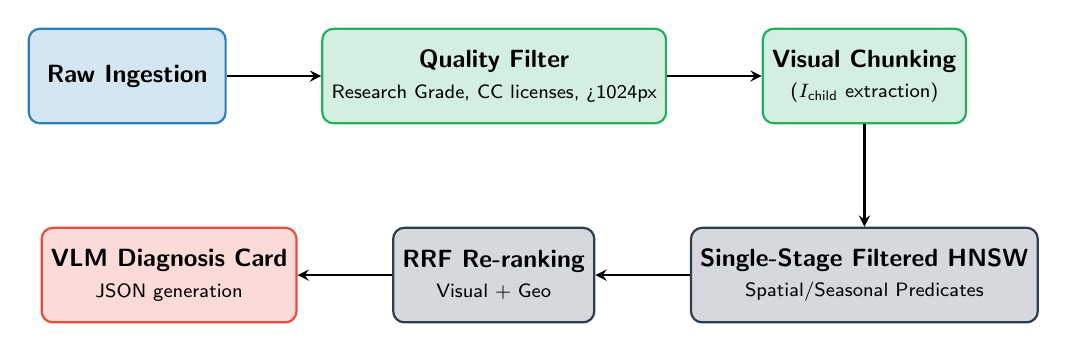
\begin{tikzpicture}[
                node distance=0.8cm and 1.2cm,
                box/.style={rectangle, draw, rounded corners, align=center, thick, fill=gray!10, minimum height=1.2cm, minimum width=2.5cm},
                arrow/.style={-stealth, thick},
                font=\small\sffamily
            ]
            \providecolor{TaxonPrimary}{RGB}{41, 128, 185}
            \providecolor{TaxonSecondary}{RGB}{39, 174, 96}
            \providecolor{TaxonDark}{RGB}{44, 62, 80}
            \providecolor{TaxonAccent}{RGB}{231, 76, 60}

            \node[box, fill=TaxonPrimary!20, draw=TaxonPrimary] (ingest) {\textbf{Raw Ingestion}};
            \node[box, fill=TaxonSecondary!20, draw=TaxonSecondary, right=of ingest] (filter) {\textbf{Quality Filter} \\ \scriptsize Research Grade, CC licenses, >1024px};
            \node[box, fill=TaxonSecondary!20, draw=TaxonSecondary, right=of filter] (chunk) {\textbf{Visual Chunking} \\ \scriptsize ($I_{\text{child}}$ extraction)};

            \node[box, fill=TaxonDark!20, draw=TaxonDark, below=of chunk, yshift=-0.5cm] (hnsw) {\textbf{Single-Stage Filtered HNSW} \\ \scriptsize Spatial/Seasonal Predicates};
            \node[box, fill=TaxonDark!20, draw=TaxonDark, left=of hnsw] (rrf) {\textbf{RRF Re-ranking} \\ \scriptsize Visual + Geo};
            \node[box, fill=TaxonAccent!20, draw=TaxonAccent, left=of rrf] (vlm) {\textbf{VLM Diagnosis Card} \\ \scriptsize JSON generation};

            \draw[arrow] (ingest) -- (filter);
            \draw[arrow] (filter) -- (chunk);
            \draw[arrow] (chunk) -- (hnsw);
            \draw[arrow] (hnsw) -- (rrf);
            \draw[arrow] (rrf) -- (vlm);
            \end{tikzpicture}
        }
    \end{center}

    \vspace{0.4cm}
    \statustarget

    \script{This diagram maps the full data flow of the MMKG pipeline. Raw data flows through strict quality filters ensuring research-grade, open-license images over 1024 pixels. Then we extract the child organism. The isolated vector is searched in our single-stage filtered HNSW index. Retrieved candidates are fused using Reciprocal Rank Fusion, and finally passed to our local VLM to emit a structured diagnosis card.}
\end{frame}

\begin{frame}{Visual Pre-Processing}{Parent-Child Visual Chunking ($I_{\text{child}}$ vs $I_{\text{parent}}$)}
    \begin{block}{Slide Topic \& Explanatory Focus}
        This slide details our visual entity chunking strategy designed to eliminate background clutter in field photography. Standard visual retrieval across uncropped citizen-science images introduces heavy noise from surrounding soil, rocks, overcast sky, or human hands holding the specimen. TaxonVision employs an upstream zero-shot detector (YOLO-World or OWL-ViT) to isolate the primary organism ($I_{\text{child}}$), to compute clean BioCLIP-2 morphological embeddings ($z_{\text{child}} \in \mathbb{R}^{768}$) without background foliage/soil noise. Simultaneously, the uncropped parent scene context ($I_{\text{parent}}$) is retained for macro-habitat and environmental verification.
    \end{block}

    \vspace{0.4cm}
    \statustarget

    \script{In nature photography, the actual insect or wildflower often takes up less than 10 percent of the frame. The rest is dirt, grass, or human fingers. If you embed the whole image, your vector captures dirt rather than biology. We use YOLO-World or OWL-ViT to detect the specimen and isolate a clean child bounding box crop for fine-grained BioCLIP-2 embedding, while preserving the parent scene image to verify environmental habitat.}
    \qa{What happens if the zero-shot detector finds multiple organisms in one image?}{Each detected child entity generates an independent bounding box and child embedding, allowing multi-organism observations to be analysed separately.}
\end{frame}

\begin{frame}{Visual Pre-Processing}{Parent-Child Visual Chunking Diagram}
    \begin{center}
        \resizebox{0.9\textwidth}{!}{
            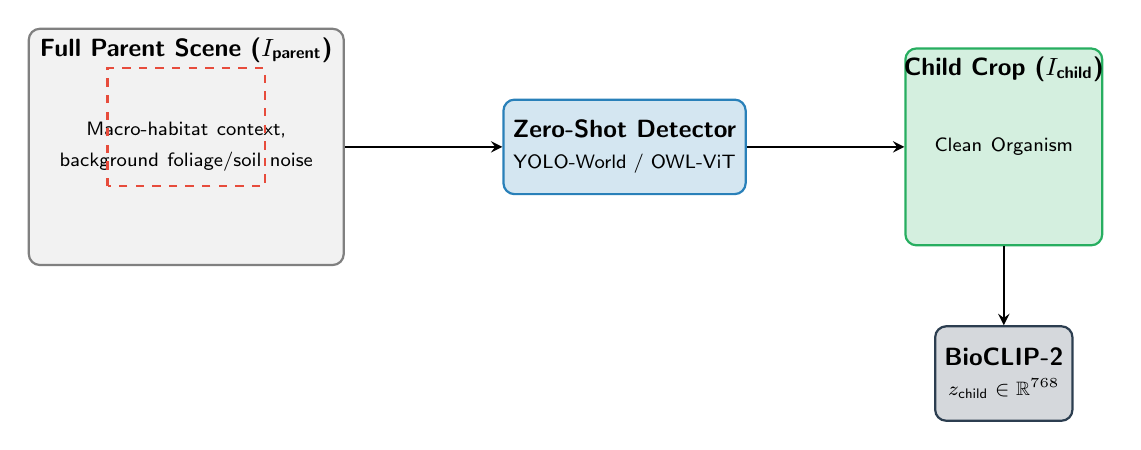
\begin{tikzpicture}[
                node distance=1.5cm,
                box/.style={rectangle, draw, rounded corners, align=center, thick, fill=gray!10, minimum height=1.2cm},
                arrow/.style={-stealth, thick},
                font=\small\sffamily
            ]
            \providecolor{TaxonPrimary}{RGB}{41, 128, 185}
            \providecolor{TaxonSecondary}{RGB}{39, 174, 96}
            \providecolor{TaxonDark}{RGB}{44, 62, 80}
            \providecolor{TaxonAccent}{RGB}{231, 76, 60}

            % Parent Image
            \node[box, fill=gray!10, draw=gray, minimum width=4cm, minimum height=3cm] (parent) {};
            \node[anchor=north, font=\small\sffamily\bfseries] at (parent.north) {Full Parent Scene ($I_{\text{parent}}$)};
            \node[anchor=center, text width=3.5cm, align=center] at (parent.center) {\scriptsize Macro-habitat context, \\ background foliage/soil noise};

            % Child Bounding Box inside Parent (conceptual)
            \draw[thick, dashed, draw=TaxonAccent] ([xshift=-1cm,yshift=-0.5cm]parent.center) rectangle ([xshift=1cm,yshift=1cm]parent.center);

            % Detector node
            \node[box, fill=TaxonPrimary!20, draw=TaxonPrimary, right=2cm of parent] (detector) {\textbf{Zero-Shot Detector} \\ \scriptsize YOLO-World / OWL-ViT};

            % Child Crop
            \node[box, fill=TaxonSecondary!20, draw=TaxonSecondary, right=2cm of detector, minimum width=2.5cm, minimum height=2.5cm] (child) {};
            \node[anchor=north, font=\small\sffamily\bfseries] at (child.north) {Child Crop ($I_{\text{child}}$)};
            \node[anchor=center, text width=2cm, align=center] at (child.center) {\scriptsize Clean Organism};

            % BioCLIP-2 Vector
            \node[box, fill=TaxonDark!20, draw=TaxonDark, below=1cm of child] (vector) {\textbf{BioCLIP-2} \\ \scriptsize $z_{\text{child}} \in \mathbb{R}^{768}$};

            \draw[arrow] (parent.east) -- (detector.west);
            \draw[arrow] (detector.east) -- (child.west);
            \draw[arrow] (child.south) -- (vector.north);

            \end{tikzpicture}
        }
    \end{center}

    \vspace{0.4cm}
    \statustarget

    \script{This diagram visually summarises the Parent-Child Visual Chunking process. We take the full parent scene containing background noise, and pass it through a zero-shot detector like YOLO-World or OWL-ViT. This extracts the child bounding box crop, separating the organism from environmental noise, which is then fed to BioCLIP-2 to compute our clean morphological embedding vector of size 768.}
\end{frame}

\begin{frame}{Biogeographical Filtering}{Single-Stage Filtered HNSW with Spatial-Temporal Predicates}
    \begin{block}{Slide Topic \& Explanatory Focus}
        This slide addresses the critical biological trap of convergent evolution—where completely unrelated species on different continents evolve near-identical morphologies (e.g., European wasp vs.\ American cicada killer). Pure visual nearest-neighbour search frequently retrieves geographically impossible candidates. TaxonVision implements single-stage filtered HNSW traversal: spatial constraints (Haversine geodesic radius $R_{\text{max}} \le 500$ km) and temporal constraints ($\Delta_{\text{season}} = 1$ month) are evaluated as boolean predicates natively inside the C++ HNSW graph walk, pruning impossible species before nearest-neighbour calculation completes.
    \end{block}

    \vspace{0.4cm}
    \statustarget

    \script{Nature is full of convergent evolution: two insects on opposite sides of the globe may look identical even though they diverged 50 million years ago. If you only look at pixels, you will misclassify a European wasp as an American cicada killer. In our HNSW vector graph, we evaluate GPS coordinates and seasonal observation month directly inside the graph traversal. If an exemplar is outside a 500-kilometre radius or wrong season, it is pruned instantly before similarity scores are computed.}
    \qa{Why not perform vector search first and filter out GPS locations afterward?}{Post-filtering suffers from candidate starvation: if your top-50 visual neighbours are all from the wrong continent, post-filtering discards all of them and leaves you with zero valid results. Native single-stage filtering guarantees high recall among geographically valid candidates.}
\end{frame}

\begin{frame}{Ensemble Ranking}{Multi-Modal Re-Ranking via Reciprocal Rank Fusion (RRF)}
    \begin{block}{Slide Topic \& Explanatory Focus}
        This slide explores how TaxonVision synthesises visual similarity and biological occurrence priors through Reciprocal Rank Fusion (RRF). After filtered HNSW retrieval yields candidate taxa, the system calculates a unified ranking score combining dense visual cosine similarity ($w_{\text{vis}} = 0.65$) with historical GBIF spatial-temporal occurrence density ($w_{\text{geo}} = 0.35$):
        \[
            \text{RRF}(d) = \frac{w_{\text{vis}}}{k + r_{\text{vis}}(d)} + \frac{w_{\text{geo}}}{k + r_{\text{geo}}(d)}
        \]
        This non-linear rank combination balances fine-grained visual evidence against ecological likelihood without requiring complex score normalisation between divergent probability distributions.
    \end{block}

    \vspace{0.4cm}
    \statustarget

    \script{Once we retrieve candidate species, how do we combine visual similarity with ecological reality? We use Reciprocal Rank Fusion. We assign a 65 percent weight to visual similarity and a 35 percent weight to historical GBIF occurrence density. Even if an exotic species looks slightly closer visually, a high local occurrence density for the native sibling species correctly tilts the ranking towards the true ecological observation.}
    \qa{What is the parameter $k$ in the RRF formula?}{The constant $k$ (typically set to 60) dampens the impact of extreme outliers at top ranks, preventing a single high rank from disproportionately dominating the final ensemble score.}
\end{frame}

\begin{frame}{Clinical-Grade Diagnosis}{VLM Context Synthesis \& Differential Diagnosis Cards}
    \begin{block}{Slide Topic \& Explanatory Focus}
        This slide details our multimodal reasoning interface for human taxonomists. When an ambiguous observation reaches triage, the query crop ($I_{\text{child}}$) and the top-3 re-ranked exemplar specimens are injected into a local Vision-Language Model (e.g., Qwen2-VL-2B). Constrained by formal grammar-based sampling, the VLM generates a structured JSON differential diagnosis card detailing distinguishing anatomical discriminators, ecological likelihoods, and CAM activation overlays. These diagnosis cards are rendered directly into Label Studio, transforming triage into rapid, high-precision expert verification.
    \end{block}

    \vspace{0.4cm}
    \statustarget

    \script{When a human taxonomist is asked to review an ambiguous specimen, we don't just dump raw images on their screen. We pass the query crop and the top-3 reference exemplars into a local Vision-Language Model like Qwen2-VL-2B. Constrained by grammar-based decoding, the VLM generates a structured JSON differential diagnosis card: it details specific anatomical discriminators, shows CAM overlays, and allows the expert to confirm the species in seconds.}
    \qa{Why use grammar-based sampling with the Vision-Language Model?}{Unconstrained VLMs hallucinate text and output unpredictable schemas. Grammar-based sampling forces the model to emit strictly valid JSON conforming to our differential diagnosis schema.}
\end{frame}

\begin{frame}{Taxonomic Agility}{Zero-Retraining Taxonomic Mutations via DuckDB}
    \begin{block}{Slide Topic \& Explanatory Focus}
        This slide examines how TaxonVision handles dynamic changes in biological taxonomy without expensive GPU model retraining. In biological science, taxonomic committees frequently alter classifications: merging species (taxonomic lumps) or dividing a single species into multiple distinct species (taxonomic splits). Because visual vectors reside in HNSW while taxonomic relationships and observation metadata reside in our decoupled DuckDB and Parquet architecture, taxonomic lumps execute as $\mathcal{O}(1)$ relational updates with zero GPU re-embedding cost. Taxonomic splits mark historical nodes with \texttt{requires\_reannotation = true}, sending them to triage before re-indexing.
    \end{block}

    \vspace{0.4cm}
    \statustarget

    \script{In real biology, taxonomy is not static. Scientists frequently merge two species into one, or split one species into three. In a standard deep learning model, every split or merge requires retraining the entire neural network from scratch. Because our architecture decouples HNSW vector storage from DuckDB relational metadata, a taxonomic merge is an instant O(1) database update. Our vectors remain untouched with zero GPU compute cost.}
    \qa{What happens during a taxonomic split when one species becomes two?}{Historical observation nodes for that taxon in DuckDB are flagged with \texttt{requires\_reannotation = true} and purged from active traversal. Their crops are routed to Label Studio for expert re-sorting, after which they are re-registered under their new respective taxon keys.}
\end{frame}


\section{Epistemic Safety \& Uncertainty}
% Chapter 7: Epistemic Safety & Mathematical Uncertainty Guarantees

\begin{frame}{Epistemic Safety}{The Illusion of Softmax Overconfidence}
    \begin{block}{Slide Topic \& Explanatory Focus}
        This slide addresses the danger of uncalibrated neural network confidence in safety-critical biological systems. Modern deep neural networks trained with cross-entropy loss are notorious for being overconfident: when presented with ambiguous images, corrupted inputs, or unseen species, the softmax activation exponentiates the largest logit, frequently outputting confidence scores $> 0.95$ on completely erroneous predictions. In ecological monitoring and toxic species identification (e.g., poisonous mushrooms), blind reliance on raw softmax leads to catastrophic misclassifications.
    \end{block}

    \vspace{0.4cm}
    \statusdone

    \script{Here is an uncomfortable truth about deep learning: softmax outputs are not probabilities! Because softmax normalizes logits exponentially, modern neural networks will happily output a 98\% confidence score on an image they have completely misclassified, or even on random noise. If a citizen science app tells a hiker that a deadly Destroying Angel mushroom is an edible field mushroom with 98\% confidence, the result is fatal. We must mathematically prevent uncalibrated overconfidence.}
    \qa{Can temperature scaling fix softmax overconfidence?}{Temperature scaling adjusts the global calibration across the dataset, but it cannot provide rigorous mathematical guarantees for individual predictions or handle out-of-distribution inputs.}
\end{frame}

\begin{frame}{Conformal Prediction}{Split Conformal Prediction \& Statistical Coverage}
    \begin{block}{Slide Topic \& Explanatory Focus}
        This slide introduces Split Conformal Prediction as our core epistemic safety framework. Unlike heuristic thresholding, conformal prediction provides a distribution-free, mathematically rigorous guarantee that the true class label $y$ will be contained within the output prediction set $C(X)$ with user-defined probability $1 - \alpha$ (e.g., $95\%$ coverage for $\alpha = 0.05$):
        \[
            P(y \in C(X)) \ge 1 - \alpha
        \]
        We explain how a held-out calibration set is used to compute non-conformity scores ($s_i = 1 - \hat{f}(x_i)_{y_i}$) and determine the empirical quantile threshold $\hat{q}$, mathematically bounding classification risk without distributional assumptions.
    \end{block}

    \vspace{0.4cm}
    \statusdone

    \script{To solve the overconfidence crisis, TaxonVision implements Split Conformal Prediction. Conformal prediction is one of the most powerful statistical techniques in modern machine learning. It guarantees—with exact mathematical proof—that if you set alpha to 0.05, the model's output prediction set will contain the true biological species at least 95 percent of the time. It requires no assumptions about the data distribution and works on top of any existing neural network.}
    \qa{What does the prediction set look like in practice?}{Instead of outputting a single fragile label, the model outputs a set of candidate labels. When the image is crystal clear, the set contains exactly one species. When the image is ambiguous, the set expands to include all statistically plausible candidate species.}
\end{frame}

\begin{frame}{Decision Making}{Dynamic Set Sizing \& Human-in-the-Loop Triage}
    \begin{block}{Slide Topic \& Explanatory Focus}
        This slide explores the operational mechanics of dynamic conformal prediction sets and automated triage routing. The cardinality of the prediction set $|C(X)|$ serves as an explicit, interpretable measure of epistemic uncertainty. When an observation produces $|C(X)| = 1$, the model has high certainty, allowing automated autonomous acceptance. When $|C(X)| > 3$ (high ambiguity) or $|C(X)| = \emptyset$ (empty set indicating extreme abnormality), the system automatically routes the observation to human taxonomist review queues, optimizing expert labor and eliminating silent model errors.
    \end{block}

    \vspace{0.4cm}
    \statusdone

    \script{In production, knowing WHEN you do not know is more valuable than making a blind guess. If our conformal prediction set has a size of 1, the model is confident and we automate the record. If the set has 6 species, or if the set is completely empty because the image violates all known feature patterns, our system flags it and routes it to our human review queue. This transforms machine learning from an autonomous liability into a trusted decision-support tool.}
    \qa{How often does an empty prediction set occur?}{Empty sets occur when the model's non-conformity score for every single known class exceeds the calibrated quantile $\hat{q}$. This typically flags corrupted files, extreme camera blur, or entirely unseen out-of-domain objects.}
\end{frame}

\begin{frame}{OOD Detection}{Energy-Based Out-of-Distribution Detection}
    \begin{block}{Slide Topic \& Explanatory Focus}
        This slide details our pre-classification safety gate: Energy-Based Out-of-Distribution (OOD) detection (\texttt{src/taxon\_vision/models/safety/ood.py}). Softmax probabilities are normalized over known classes and cannot reliably detect when an image does not belong to ANY known biological category (e.g., an indoor living room, vehicle, or macro photograph of rock mineral). Energy-based scores compute the negative Helmholtz free energy of the un-normalized logits:
        \[
            E(x; f) = -T \cdot \log \sum_{i=1}^K e^{f_i(x) / T}
        \]
        Observations with energy exceeding the calibrated threshold are immediately flagged as OOD prior to inference.
    \end{block}

    \vspace{0.4cm}
    \statusdone

    \script{What happens if someone points the biodiversity camera at a parked car or a coffee cup? A standard classifier will force that car into one of its biological classes, perhaps declaring it a 'Black Bear' with high confidence. To prevent this, we run an Energy-Based OOD detector on the raw logits before classification. Low energy indicates biological in-distribution features, while high energy flags non-biological anomalies before they can corrupt downstream records.}
    \qa{Why is energy score superior to maximum softmax probability for OOD detection?}{Softmax normalization destroys logit magnitude information due to the denominator sum. The energy function maps directly to the Helmholtz free energy and aligns with the true data density, making it far more sensitive to abnormal feature spaces.}
\end{frame}

\begin{frame}{Model Explainability}{Forward-Hooked Class Activation Mapping ($<2$ ms)}
    \begin{block}{Slide Topic \& Explanatory Focus}
        This slide presents our production-grade explainability subsystem: forward-hooked Class Activation Mapping (CAM / Eigen-CAM). In ecological validation, taxonomists must verify that the model is identifying genuine diagnostic morphological features (such as petal shape or antennae structure) rather than relying on spurious background correlations (such as garden fences or photo watermarks). Standard Grad-CAM requires a backward pass that doubles latency. By utilizing forward hooks on penultimate feature activations, our implementation generates visual saliency heatmaps in under 2 milliseconds without backward gradient overhead.
    \end{block}

    \vspace{0.4cm}
    \statusdone

    \script{Machine learning models are notorious for learning the wrong shortcuts. In one famous case, a husky classifier actually learned to detect snow in the background rather than the dog. To prove to taxonomists that our model looks at biological traits, we generate Class Activation Maps. By using PyTorch forward hooks on our feature extractor, we compute saliency heatmaps in less than 2 milliseconds on the GPU, completely bypassing the heavy backward pass required by older Grad-CAM algorithms.}
    \qa{Can forward-hooked CAM be served in real-time to mobile users?}{Yes. Because it takes under 2 milliseconds, the visual heatmap overlay is returned in the exact same HTTP response as the classification set without impacting user experience.}
\end{frame}


\section{CI/CD \& Kubernetes Deployment}
% Chapter 8: CI/CD, Containerization & Kubernetes Deployment

\begin{frame}{CI/CD Architecture}{Dual Workflow: GitHub Actions Cloud vs Jenkins Bare-Metal}
    \begin{block}{Slide Topic \& Explanatory Focus}
        This slide examines our production CI/CD architecture, explaining the strategic division between cloud-hosted GitHub Actions and on-premise Jenkins CD. Public pull requests cannot be granted direct network or SSH access to private bare-metal GPU clusters without creating extreme security risks. Instead, GitHub Actions executes cloud-based static analysis gates (Ruff linting, Mypy typing, cyclomatic complexity, license compliance, OKF validation). Once PRs are verified and merged into \texttt{develop} or \texttt{main}, Jenkins on \texttt{hive-mind} triggers bare-metal deployment, container builds, and GPU integration testing within isolated Kubernetes pods.
    \end{block}

    \vspace{0.4cm}
    \statusdone

    \script{Here is an enterprise DevOps pattern every student must learn: how do you connect cloud GitHub to private bare-metal servers securely? You never allow GitHub Actions to SSH directly into your private GPU cluster; that would create a massive security vulnerability. Instead, GitHub Actions runs fast cloud checks—linting, typing, and licensing—on public runners. Once code is approved, Jenkins running inside our private network pulls the signed commit and executes deployment locally.}
    \qa{Why not use GitHub Self-Hosted Runners directly on hive-mind?}{Self-hosted runners on public or shared repos can execute untrusted code from malicious pull requests directly on your physical host machine. Ephemeral Jenkins agent pods isolate every job inside disposable container sandboxes.}
\end{frame}

\begin{frame}{Code Quality}{Cognitive Complexity Gates: complexipy $\le 15$ \& Strict Typing}
    \begin{block}{Slide Topic \& Explanatory Focus}
        This slide explores the software engineering principles enforced across our Python codebase. Machine learning codebases often degrade into unmaintainable ``research spaghetti'' filled with deeply nested loops, global state, and un-typed tensors. TaxonVision enforces strict automated gates: Ruff for formatting and linting, Mypy for static type verification, and \texttt{complexipy} enforcing a strict cognitive complexity limit of $\le 15$ per function. Functions exceeding this threshold are rejected at pre-commit, forcing modular refactoring, helper extraction, and clean architecture.
    \end{block}

    \vspace{0.4cm}
    \statusdone

    \script{Why do so many data science projects fail when moving to production? Code complexity. In Jupyter notebooks, people write 300-line functions with 6 nested loops and zero type annotations. In TaxonVision, our CI gate uses \texttt{complexipy} to measure cognitive complexity. If any function scores higher than 15, the build fails instantly. This forces engineers to write modular, single-responsibility functions that are easy to unit test and maintain.}
    \qa{What was an example of a refactoring forced by this complexity rule?}{In \texttt{runner.py}, our embedding split preparation and index mapping functions originally scored above 20 due to combined dictionary parsing and tensor slicing. We decomposed them into dedicated helper methods, bringing complexity down to 6.}
\end{frame}

\begin{frame}{Containerization}{Multi-Stage Docker Architecture \& GHCR OCI Registry}
    \begin{block}{Slide Topic \& Explanatory Focus}
        This slide covers production containerization using multi-stage Docker builds published to GitHub Container Registry (GHCR). Naïve Docker images package full compiler toolchains, package caches, and test fixtures, bloating images to $> 10$ GB. Our multi-stage build uses an isolated builder stage to resolve Pixi dependencies and compile extensions, copying only the minimal runtime artifacts into the final production image. This reduces final image sizes to $< 1.5$ GB, accelerates Kubernetes pod startup times, and minimizes the security attack surface.
    \end{block}

    \vspace{0.4cm}
    \statusdone

    \script{In production, your deployment artifact is a container image. A novice Dockerfile copies the entire workspace and runs 'pip install', resulting in an 8-gigabyte bloated container full of build tools and temporary files. Our multi-stage Dockerfile builds dependencies in a disposable stage and copies only the compiled runtime binaries into the final image. This cuts our image down to under 1.5 gigabytes and makes Kubernetes pod deployments lightning-fast.}
    \qa{Why do we push images to GitHub Container Registry (GHCR)?}{GHCR provides authenticated, versioned OCI storage integrated directly with our GitHub repository permissions and release tags, serving as our single source of truth for deployment artifacts.}
\end{frame}

\begin{frame}{Cluster Orchestration}{Lightweight Kubernetes (k3s) \& Ephemeral Pods}
    \begin{block}{Slide Topic \& Explanatory Focus}
        This slide details our bare-metal cluster management using k3s, a certified lightweight Kubernetes distribution optimized for edge and single-node enterprise clusters. We discuss how Jenkins dynamically provisions ephemeral agent pods inside the cluster to execute build pipelines, mounting local NVMe Rattler package caches to eliminate redundant network downloads. Once the pipeline job completes, the agent pod is automatically destroyed, ensuring complete environmental cleanliness without lingering processes or zombie CUDA allocations.
    \end{block}

    \vspace{0.4cm}
    \statusdone

    \script{On our bare-metal server, we run k3s—a lightweight, highly efficient Kubernetes distribution. When Jenkins receives a build webhook, it doesn't run the job on the host OS. Instead, it spins up an ephemeral agent container pod inside k3s, executes the build with local NVMe caching, and terminates the pod immediately. This guarantees that every single build starts in a pristine, reproducible environment with zero leftover state.}
    \qa{Why use k3s instead of standard k8s on a single bare-metal node?}{Standard Kubernetes runs dozens of heavy control-plane components that consume gigabytes of RAM. k3s packages the entire control plane into a single binary consuming under 512 megabytes of RAM, reserving maximum system memory for our models.}
\end{frame}

\begin{frame}{Deployment Strategy}{Zero-Downtime Rolling Updates \& Health Probes}
    \begin{block}{Slide Topic \& Explanatory Focus}
        This slide illustrates our zero-downtime deployment strategy in Kubernetes. Updating an inference service must never drop active HTTP connections or return 502 Bad Gateway errors to clients. We configure Kubernetes Deployment manifests with readiness and liveness probes targeting FastAPI \texttt{/health} endpoints. When a new container image is deployed, Kubernetes waits for model weights to load and warm up in memory before switching incoming Traefik ingress traffic, terminating older replica pods only after new pods are fully serving traffic.
    \end{block}

    \vspace{0.4cm}
    \statusdone

    \script{Imagine updating your model in production: if you kill the old container before the new one finishes loading its 500-megabyte neural network into GPU memory, all incoming user requests fail with 500 errors. We configure Kubernetes rolling updates with readiness probes. The ingress keeps sending traffic to the old model until the new model reports that its weights are warmed up and ready. The switch happens seamlessly with zero dropped requests.}
    \qa{What is the difference between a liveness probe and a readiness probe?}{A liveness probe checks if the process is alive; if it fails, Kubernetes restarts the pod. A readiness probe checks if the pod is ready to accept HTTP traffic; if it fails, traffic is diverted without killing the container.}
\end{frame}


\section{Observability \& Active Learning}
% Chapter 9: Observability, Drift Monitoring & Active Learning

\begin{frame}{Observability}{Production Telemetry: Prometheus Metrics \& Grafana}
    \begin{block}{Slide Topic \& Explanatory Focus}
        This slide covers production observability and real-time telemetry. In MLOps, monitoring goes far beyond standard HTTP 200/500 error counts. Our FastAPI serving service exposes a \texttt{/metrics} endpoint scraped by Prometheus, capturing domain-specific metrics: p50/p95/p99 inference latency, GPU memory utilization, energy-based OOD detection rates, prediction set cardinality distribution, and human triage escalation ratios. Grafana dashboards visualize these metrics in real-time, enabling operators to detect system degradation before users notice.
    \end{block}

    \vspace{0.4cm}
    \statusdone

    \script{Observability in MLOps is fundamentally different from traditional DevOps. In web development, you monitor CPU and HTTP status codes. In MLOps, an API can return HTTP 200 OK all day while predicting complete nonsense! We monitor domain-specific metrics: average conformal prediction set size, percentage of samples routed to human review, and OOD energy distributions. If average set size jumps from 1.2 to 4.5, we know immediately that the data distribution has shifted.}
    \qa{How does Prometheus scrape metrics from our service?}{FastAPI instruments latency and counters using the \texttt{prometheus\_client} library, exposing a \texttt{/metrics} endpoint that the Prometheus server polls every 15 seconds.}
\end{frame}

\begin{frame}{Drift Monitoring}{Data \& Concept Drift: Wasserstein-1 Distance vs MMD}
    \begin{block}{Slide Topic \& Explanatory Focus}
        This slide explores statistical drift detection across high-dimensional feature spaces (\texttt{src/taxon\_vision/observability/drift.py}). As seasons change, flora blooms, or new mobile cameras enter the field, input distributions drift away from training baselines. We contrast 1D marginal statistical tests (such as Kolmogorov-Smirnov or 1D Wasserstein-1 distance across individual feature projections) with full-manifold multivariate metrics like Maximum Mean Discrepancy (MMD) with RBF kernels. When drift exceeds calibrated statistical thresholds, automated alerts trigger the retraining pipeline.
    \end{block}

    \vspace{0.4cm}
    \statusdone

    \script{Machine learning models degrade over time because the real world changes—we call this data drift. If autumn arrives, leaves turn yellow and lighting shifts, but our training set was collected in summer. We use the Wasserstein-1 Earth Mover's Distance to monitor the distribution of incoming feature embeddings against our baseline training distribution. When the statistical distance crosses our alert threshold, the system flags the drift and prepares an active learning cycle.}
    \qa{Why not run multivariate MMD on every single incoming inference request?}{Computing full-manifold MMD across high-dimensional embeddings has quadratic complexity $O(N^2)$ in sample size. We perform 1D Wasserstein distance on projected features in real time and reserve full MMD for periodic offline batch audits.}
\end{frame}

\begin{frame}{Active Learning}{Active Learning: BADGE Sampling \& Human Review Queue}
    \begin{block}{Slide Topic \& Explanatory Focus}
        This slide presents our active learning subsystem: the BADGE (Batch Active learning by Diverse Gradient Embeddings) query strategy and human triage interface. When thousands of unlabelled field observations stream in, random sampling or pure uncertainty sampling yields redundant, low-diversity annotations. BADGE computes hypothetical gradient embeddings representing both epistemic uncertainty and feature diversity, selecting the most informative batch via $k$-MEANS++. These priority samples are pushed to Label Studio for expert verification, closing the feedback loop.
    \end{block}

    \vspace{0.4cm}
    \statuspartial

    \script{Annotation by expert taxonomists is expensive and slow. If you send them 10,000 photos of the same common dandelion, you waste their time. BADGE solves this by analyzing the gradients that each unlabelled image would induce in the model. It uses k-MEANS++ clustering in gradient space to pick a batch of images that are both highly uncertain AND visually diverse. This maximizes the model's accuracy improvement per dollar spent on human labeling.}
    \qa{What is the current status of the active learning pipeline?}{The BADGE mathematical sampling algorithm and Label Studio export formats are fully implemented in \texttt{src/taxon\_vision/active\_learning/badge.py}. The automated webhook that triggers unattended model retraining upon annotation completion is our Phase 3 target milestone.}
\end{frame}


\section{Roadmap \& Engineering Lessons}
% Chapter 10: Roadmap, Delivery Phases & Pedagogical Takeaways

\begin{frame}{Project Roadmap}{Implementation Status vs Architectural Roadmap}
    \begin{block}{TaxonVision Delivery Phases}
        An honest, transparent breakdown of the current implementation status versus future architectural milestones.
        \begin{itemize}
            \item \textbf{Phase 1 (Foundation):} Complete. Pixi toolchain, DVC/S3 streaming, pre-commit gates, license compliance.
            \item \textbf{Phase 2 (Model \& MLOps):} Complete. Frozen feature extraction, Class-Balanced Loss, Optuna, Conformal safety, k3s, GHCR, Jenkins.
            \item \textbf{Phase 3 (Continuous Intelligence):} Target. Full Milvus MMKG, Vision-RAG, Label Studio retraining trigger.
        \end{itemize}
    \end{block}

    \begin{center}
    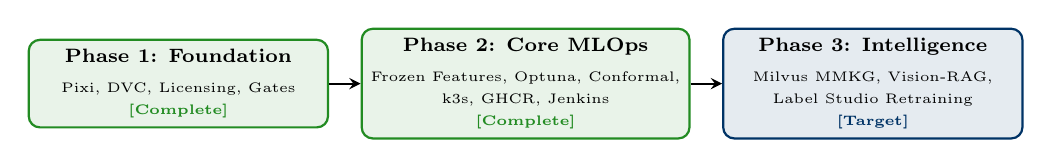
\begin{tikzpicture}[
        node distance=0.4cm and 0.4cm,
        box/.style={rectangle, draw, rounded corners, align=center, minimum height=1.1cm, minimum width=3.8cm, font=\scriptsize},
        arrow/.style={-stealth, thick},
        done/.style={fill=plantgreen!10, draw=plantgreen, thick},
        target/.style={fill=deepblue!10, draw=deepblue, thick}
    ]
        % Nodes
        \node[box, done] (phase1) {
            \textbf{Phase 1: Foundation}\\[1mm]
            \tiny Pixi, DVC, Licensing, Gates\\
            \tiny \textcolor{plantgreen}{\textbf{[Complete]}}
        };

        \node[box, done, right=of phase1] (phase2) {
            \textbf{Phase 2: Core MLOps}\\[1mm]
            \tiny Frozen Features, Optuna, Conformal,\\
            \tiny k3s, GHCR, Jenkins\\
            \tiny \textcolor{plantgreen}{\textbf{[Complete]}}
        };

        \node[box, target, right=of phase2] (phase3) {
            \textbf{Phase 3: Intelligence}\\[1mm]
            \tiny Milvus MMKG, Vision-RAG,\\
            \tiny Label Studio Retraining\\
            \tiny \textcolor{deepblue}{\textbf{[Target]}}
        };

        % Arrows
        \draw[arrow] (phase1) -- (phase2);
        \draw[arrow] (phase2) -- (phase3);

    \end{tikzpicture}
    \end{center}

    \script{Let's review our progress transparently. Phase 1 and Phase 2 are complete and battle-tested in our repository today: our reproducible Pixi environment, S3 zero-copy streaming, Class-Balanced Loss runner, conformal safety bounds, Jenkins container builds, and Kubernetes manifests are live. Phase 3—connecting the Milvus vector database into our active learning webhook loop—is our ongoing target architecture roadmap.}
    \qa{How do we ensure that new feature development does not regress existing Phase 1 and 2 capabilities?}{Every commit is protected by our pre-commit gates, automated test fixtures in \texttt{tests/}, and CI pipeline validation including license and complexity audits.}
\end{frame}

\begin{frame}{Pedagogical Takeaways}{Classic MLOps Anti-Patterns \& Engineering Fixes}
    \begin{block}{Bootcamp vs. Enterprise}
        Core pedagogical lessons for transitioning into MLOps, contrasting common junior anti-patterns with enterprise architectural solutions.
    \end{block}

    \begin{center}
    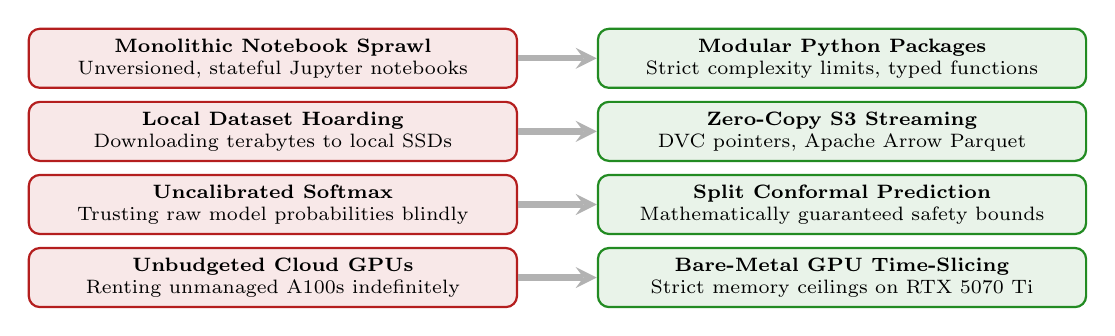
\begin{tikzpicture}[
        node distance=0.15cm and 0.5cm,
        box/.style={rectangle, draw, rounded corners, align=center, minimum height=0.75cm, minimum width=6.2cm, font=\scriptsize},
        bad/.style={fill=herbired!10, draw=herbired, thick},
        good/.style={fill=plantgreen!10, draw=plantgreen, thick},
        arrow/.style={-stealth, thick, line width=0.8mm, draw=black!30}
    ]
        % Row 1
        \node[box, bad] (bad1) {\textbf{Monolithic Notebook Sprawl}\\Unversioned, stateful Jupyter notebooks};
        \node[box, good, right=1cm of bad1] (good1) {\textbf{Modular Python Packages}\\Strict complexity limits, typed functions};
        \draw[arrow] (bad1) -- (good1);

        % Row 2
        \node[box, bad, below=of bad1] (bad2) {\textbf{Local Dataset Hoarding}\\Downloading terabytes to local SSDs};
        \node[box, good, right=1cm of bad2] (good2) {\textbf{Zero-Copy S3 Streaming}\\DVC pointers, Apache Arrow Parquet};
        \draw[arrow] (bad2) -- (good2);

        % Row 3
        \node[box, bad, below=of bad2] (bad3) {\textbf{Uncalibrated Softmax}\\Trusting raw model probabilities blindly};
        \node[box, good, right=1cm of bad3] (good3) {\textbf{Split Conformal Prediction}\\Mathematically guaranteed safety bounds};
        \draw[arrow] (bad3) -- (good3);

        % Row 4
        \node[box, bad, below=of bad3] (bad4) {\textbf{Unbudgeted Cloud GPUs}\\Renting unmanaged A100s indefinitely};
        \node[box, good, right=1cm of bad4] (good4) {\textbf{Bare-Metal GPU Time-Slicing}\\Strict memory ceilings on RTX 5070 Ti};
        \draw[arrow] (bad4) -- (good4);

    \end{tikzpicture}
    \end{center}

    \script{For all of you in this course, if you take away four key lessons from this project, make it these four: First, stop writing monolithic notebooks—use modular packages with strict complexity limits. Second, don't download multi-terabyte datasets locally—stream them and cache embeddings. Third, never trust raw softmax probabilities—use conformal prediction sets for safety. And fourth, don't waste thousands of dollars on unmanaged cloud GPUs—budget your VRAM and use time-slicing.}
    \qa{What is the fastest way for a junior data scientist to adopt these best practices?}{Start by enforcing automated pre-commit hooks with Ruff and Mypy, tracking datasets with DVC, and writing unit tests for your data transformation functions before touching model code.}
\end{frame}

\begin{frame}{Conclusion}{Core Architectural Principles \& System Vision}
    \begin{block}{The Pillars of Production Systems Engineering}
        TaxonVision is built on three uncompromising principles that define enterprise MLOps.
        \begin{itemize}
            \item \textbf{Reproducibility by Default:} Using Pixi environments, DVC data lineage, and declarative k3s manifests ensures every run is perfectly replicable.
            \item \textbf{Mathematical Safety under Uncertainty:} Split Conformal Prediction guarantees error bounds, refusing confident misclassification.
            \item \textbf{Hardware-Conscious Sustainability:} Bare-metal GPU time-slicing, INT8 ONNX quantization, and zero-allocation inference maximize throughput per watt.
        \end{itemize}
    \end{block}

    \vspace{0.4cm}
    \statusdone

    \script{To conclude: MLOps is not just about using trendy tools like Kubernetes or Docker. It is a systems engineering mindset. It means building models that are reproducible down to the exact commit, mathematically honest about what they don't know, and engineered to run reliably on physical hardware within budget. TaxonVision proves that with the right architecture, we can tackle the most complex biodiversity challenges on Earth with mathematical confidence and operational excellence. Thank you!}
    \qa{Where can students inspect the source code and documentation?}{The entire repository, including Zensical documentation, LaTeX strategy reports, and CI/CD pipelines, is maintained under strict version control in the taxon-vision-mlops repository.}
\end{frame}


\end{document}
